I used the $3\times3$ Prewitt filter to produce image dipicting the edges in the original image:

$$\delta_x = \frac{1}{3}
\begin{bmatrix}
    -1 & 0 & 1 \\
    -1 & 0 & 1 \\
    -1 & 0 & 1
\end{bmatrix}$$

and,

$$\delta_y = \frac{1}{3}
\begin{bmatrix}
-1 & -1 & -1 \\
0 & 0 & 0 \\
1 & 1 & 1
\end{bmatrix}$$

These filters when convolved with the original image gives the following images:

\begin{figure}[H]
    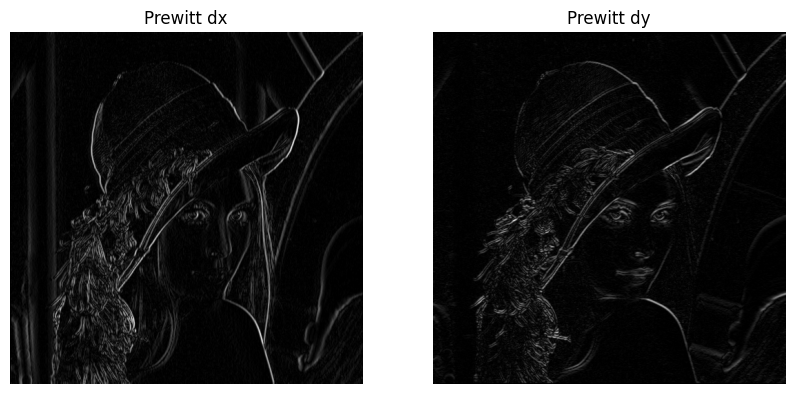
\includegraphics[width=1.06\textwidth]{res/1_prewitt.png}
    \caption{Prewitt filter applied to the original image}\label{fig:1_prewitt}
\end{figure}

Here we notice that the images is highlighting the edges that were in the orignial image.

\textbf{Comparision with larger filter (5 by 5)}

I used the following $5\times5$ filter to produce image dipicting the edges in the original image:

$$\delta_x = \frac{1}{15}
\begin{bmatrix}
-1 & -2 & 0 & 2 & 1 \\
-1 & -2 & 0 & 2 & 1 \\
-1 & -2 & 0 & 2 & 1 \\
-1 & -2 & 0 & 2 & 1 \\
-1 & -2 & 0 & 2 & 1
\end{bmatrix}$$

and,

$$\delta_y = \frac{1}{15}
\begin{bmatrix}
-1 & -1 & -1 & -1 & -1 \\
-2 & -2 & -2 & -2 & -2 \\
0 & 0 & 0 & 0 & 0 \\
2 & 2 & 2 & 2 & 2 \\
1 & 1 & 1 & 1 & 1
\end{bmatrix}$$

Here the 2nd and 2nd last enteries have greater value than the first and the last enteries. This is because the center pixel has more weightage than the pixels at the corners. This is done to increase localization in the gradient.

\begin{figure}[H]
    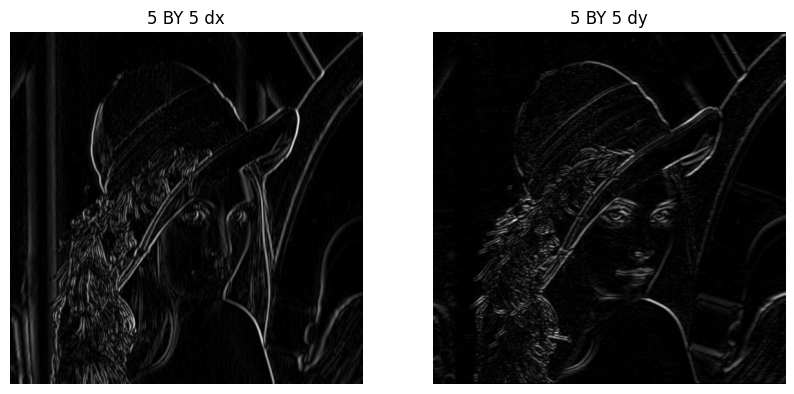
\includegraphics[width=1.06\textwidth]{res/1_5_by_5.png}
    \caption{5 by 5 filter applied to the original image}\label{fig:1_5by5}
\end{figure}

\textbf{Results}

The $\delta_x$ filter detects vertical edges and the $\delta_y$ filter detects horizontal edges. This is happening because the filter computes gradient about the direction mentioned in its subscript. So when there is sudden change in the pixel values in the direction of the filter, the filter gives a high value. Since edges are nothing but sudden changes in a function. This is why the edges are highlighted in the images.

Few differences observed between different size of filters:

\begin{itemize}
    \item The edges are thicker in $5\times5$ than in $3\times3$.
    \item $3\times3$ does a lot better in preserving the hair details.
\end{itemize}